
\subsection[SO*(2n)]{$\mathrm{SO}^*(2n) \sim D_n, n\geq 4$}

\subsubsection{Root system data}

\[\alpha_i = \epsilon_i - \epsilon_{i+1}, i<n, \alpha_n = \epsilon_{n-1} + \epsilon_n\]
\[\omega_i = \epsilon_1+\cdots \epsilon_i, i < n-1, \quad \omega_{n-1} = \frac{1}{2}(\epsilon_1 + \cdots \epsilon_{n-1}-\epsilon_n), \quad \omega_{n} = \frac{1}{2}(\epsilon_1 + \cdots \epsilon_{n-1}+\epsilon_n)\]
\begin{align*}
 \roots &= \{ \pm \epsilon_i \pm \epsilon_j | i\neq j, i,j = 1\ldots n \} \\
 \roots_c^+ &= \{ \epsilon_i-\epsilon_j | 1\leq i < j \leq  n\}\\
 \roots_n^+ &= \{ \epsilon_i + \epsilon_j | 1 \leq i <  j \leq n \}
\end{align*}
\[\beta = \epsilon_1+\epsilon_2,\quad \rho = (n-1,\ldots ,1,0),\quad \zeta = \frac{1}{2}(1,1,\ldots,1)\]
\inserttikzfigure{diagrams/dynkin_Dn_n.tikz}{Marked Dynkin diagram for $\mathrm{SO}^*(2n)$}

\begin{center}\begin{threeparttable}
\begin{tabular}{CCCCC}
  \text{Vertex } \lambda_a & \text{Weight } \mu_a &  Q(\lambda_a) = R(\lambda_a)& l(\lambda_a) \\ \hline
  \omega_2 - (2n-2)\omega_n & -(2n-2)\omega_n & \mathrm{SU}(1,1) &  1 \\
  \omega_p -2(n-p+l) \omega_n & \omega_{p-2l}-2(n-p+l)\omega_n & \mathrm{SO}^*(2p)\tnote{1} & 1\leq l \leq \floor{\frac{p}{2}} \\
  \omega_{n-1} - (1+2l)\omega_n & \omega_{n-1-2l} - 2(1+l)\omega_n &  \mathrm{SO}^*(2n-2) & 1\leq l \leq \floor{\frac{n-1}{2}} \\
  -(2l-2)\omega_n & \omega_{n-2l} - 2l\omega_n &  \mathrm{SO}^*(2n)  & 1\leq l \leq \floor{\frac{n}{2}} \\
  \omega_1 +\omega_{q+1} - (2n-q)\omega_n & \omega_q -(2n-q)\omega_n & \mathrm{SU}(1,q)\tnote{2} & 1\\
  \omega_1 +\omega_{n-1} - (n+1)\omega_n & \omega_{n-2} - (n+2)\omega_n &  \mathrm{SU}(1,n-2)  & 1 \\
  \omega_1 -(n-1)\omega_n & \omega_{n-1} - n\omega_n &  \mathrm{SU}(1,n-1)  & 1
\end{tabular}
\smallskip
\begin{tablenotes}
 \item [1] $3 \leq p \leq n-2$
 \item [2] $2 \leq q \leq n-3$
\end{tablenotes}\caption{Vertices and root systems for $\mathrm{SO}^*(2n)$, $n\geq 4$}
\end{threeparttable}\end{center}

Let $a=(Q,R,l)$, $Q=R$. Then for $R=\mathrm{SO}^*(2p)$, $3\leq p\leq n$
\[
 C_a = \{a_p\omega_p+\cdots + a_n\omega_n \,|\, a_n = -2a_p - \cdots -2a_{n-2} - a_{n-1}\}
\]
and for  $R=\mathrm{SU}(1,q)$, $1\leq q \leq n-1$
\[
 C_a = \{a_1\omega_1 + a_{q+1}\omega_{q+1} + \cdots + a_n\omega_n \,|\, a_n = -(a_1 + 2a_{q+1} + \cdots + 2a_{n-2} + a_{n-1})\}.
\]

\subsubsection{Nilpotent cohomology in detail}

Scalar products of positive noncompact roots with $\rho$ are
\[
 (\epsilon_i + \epsilon_j, \rho) = 2n - i -j.
\]

\begin{enumerate}
 \item $\lambda =  \omega_2 - (2n-2)\omega_n $\\
  \[
   (\epsilon_i + \epsilon_j,\lambda+\rho) = \begin{cases}
                                             1, &  i=1,j=2 \\
                                             2-j, & i=1, 2 < j \leq n\\
                                             1-j, & i=2, 2 < j \leq n \\
                                             2-i-j, & 2 < i < j
                                            \end{cases}
  \]
  \[
   \Psi^+_\lambda = \emptyset, \quad \roots^+_{n,\lambda} = \{ \epsilon_1 + \epsilon_2 \}
  \]

 \item $\lambda = \omega_p -2(n-p+l) \omega_n$, $3\leq p \leq n-2$, $1\leq l \leq \floor{\frac{p}{2}}$\\
  \[
   (\epsilon_i + \epsilon_j,\lambda+\rho) = \begin{cases}
                                             2(p-l+1)-i-j, & 1\leq i < j \leq p \\
                                             2(p-l)+1-i-j, & 1 \leq i \leq p < j \leq n\\
                                             2(p-l)-i-j, &  p <i < j \leq n
                                            \end{cases}
  \]
  \begin{multline*}
   \Psi^+_\lambda = \{ \epsilon_i + \epsilon_{2(p-l)+1-i} \,|\, \max\{1,1+2(p-l)-n\} \leq i < p-2l+1 \} \cup \\  \{ \epsilon_i + \epsilon_{2(p-l)+2-i} \,|\, p-2l+2 \leq i < p-l+1 \}
  \end{multline*}
  \begin{multline*}
   (\Psi^+_\lambda)^\perp \supseteq \{ \epsilon_i + \epsilon_j \,|\, \\ i,j \in \{ 1,\ldots,\max\{0,2(p-l)-n\},p-2l+1,p-l+1,\min\{ 2(p-l),n \}+1.\ldots,n \} \}
  \end{multline*}
  \[
   \roots^+_{n,\lambda} = \{ \}
  \]

  
 \item $\lambda = \omega_{n-1} - (1+2l)\omega_n  $, $  1\leq l \leq \floor{\frac{n-1}{2}}$  \\
  \[
   (\epsilon_i + \epsilon_j,\lambda+\rho) = \begin{cases}
                                             2(n-l)-i-j, & 1 \leq i<	j < n \\
                                             n-2l-1-i, & 1 \leq i< n = j
                                            \end{cases}
  \]
  \begin{enumerate}
   \item $n$ is odd and $l=\frac{n-1}{2}$\\
    \[
      \Psi^+_\lambda = \Big\{\epsilon_i + \epsilon_{n+1-i} \,\big|\, 1<i< \frac{n+1}{2} \Big\}
    \]
    \[
      \roots^+_{n,\lambda} = \left\{ \epsilon_1 + \epsilon_{\frac{n+1}{2}} \right\}
    \]
    
   \item $n$ even or $n$ odd and $l < \frac{n-1}{2}$\\
    \[
      \Psi^+_\lambda = \{\epsilon_i + \epsilon_{2(n-l)-i} \,|\, n-2l<i<n-l \} \cup \{ \epsilon_{n-2l-1} + \epsilon_n \}
    \]
    \[
      \roots^+_{n,\lambda} = \{ \epsilon_i + \epsilon_j \,|\, i < j \et i,j\in \{1,\ldots,n-2l-2,n-2l,n-l\} \}
    \]
  \end{enumerate}
  
 \item $\lambda = -(2l-2)\omega_n $, $ 1\leq l \leq \floor{\frac{n}{2}} $\\
 \[
  (\epsilon_i + \epsilon_j,\lambda+\rho) = 2(n-l+1)-i-j
 \]
 \[
  \Psi^+_\lambda = \{ \epsilon_i + \epsilon_{2(n-l+1)-i} \,|\, n + 2(1-l) \leq i \leq n-l  \} 
 \]
 \[
  \roots^+_{n,\lambda} =  \{ \epsilon_i + \epsilon_j \,|\, i < j \et i,j \in \{ 1,\ldots, n-2l+1,n-l+1 \} \}
 \]

 
 \item $\lambda =  \omega_1 +\omega_{q+1} - (2n-q)\omega_n$, $ 2\leq q \leq n-3$\\
  \[
   (\epsilon_i + \epsilon_j,\lambda+\rho) = \begin{cases}
                                             2+q-j, & i = 1, 2\leq j \leq q+1 \\
                                             1+q-j, & i = 1, q+1 < j \leq n \\
                                             2+q-i-j, & 2\leq i < j \leq q+1 \\ % here are the only singular roots
                                             1+q-i-j, & 2\leq i \leq q+1 < j \leq n \\
                                             q-i-j, &   q+1 < i < j \leq n \\
                                            \end{cases}
  \]
  \[
   \Psi^+_\lambda = \Big\{ \epsilon_i + \epsilon_{2+q-i} \,\big|\, 1 < i < \frac{q}{2}+1 \Big\}
  \]
  \[
   \roots^+_{n,\lambda} = \begin{cases}
                           \{ \epsilon_1 + \epsilon_{q+1}  \}, & q \text{ is odd}\\
                           \big\{ \epsilon_1 + \epsilon_{q+1}, \epsilon_1 + \epsilon_{\frac{q}{2}+1}   \big\}, & q \text{ is even}
                          \end{cases}
  \]
  
 \item $\lambda = \omega_1 +\omega_{n-1} - (n+1)\omega_n $\\
  \[
   (\epsilon_i + \epsilon_j,\lambda+\rho) = \begin{cases}
                                             n - j, & i = 1 < j < n \\
                                             -1, & i = 1, j=n\\
                                             n-i-j, & 1 < i < j < n\\
                                             -1-i, & 1 < i < n = j
                                            \end{cases}
  \]
  \[
   \Psi^+_\lambda = \Big\{ \epsilon_i + \epsilon_{n-i} \,\big|\, 1 < i < \frac{n}{2}\Big\}, \quad 
   \roots^+_{n,\lambda} = \begin{cases}
				\{\epsilon_1 + \epsilon_{n-1} \}, & n \text{ is odd} \\
				\{\epsilon_1 + \epsilon_{n-1}, \epsilon_1 + \epsilon_{\frac{n}{2}} \}, & n \text{ is even}
			  \end{cases}
  \]
  
 \item $\lambda = \omega_1 -(n-1)\omega_n $\\
 \[
  (\epsilon_i + \epsilon_j,\lambda+\rho) = \begin{cases}
                                            n+1-j, & i=1<j\leq n\\
                                            n+1-i-j, & 1<i<j\leq n
                                           \end{cases}
 \]
 \[
   \Psi^+_\lambda = \Big\{\epsilon_i + \epsilon_{n+1-i} \,\big|\, 1 < i < \frac{n+1}{2} \Big\}
 \]
 \[
   \roots^+_{n,\lambda} = \begin{cases}
				\{\epsilon_1 + \epsilon_n \}, & n \text{ is even} \\
				\{\epsilon_1 + \epsilon_n, \epsilon_1 + \epsilon_{\frac{n+1}{2}} \}, & n \text{ is odd}
			  \end{cases}
  \]
\end{enumerate}

\begin{figure}[H]
  \centering
  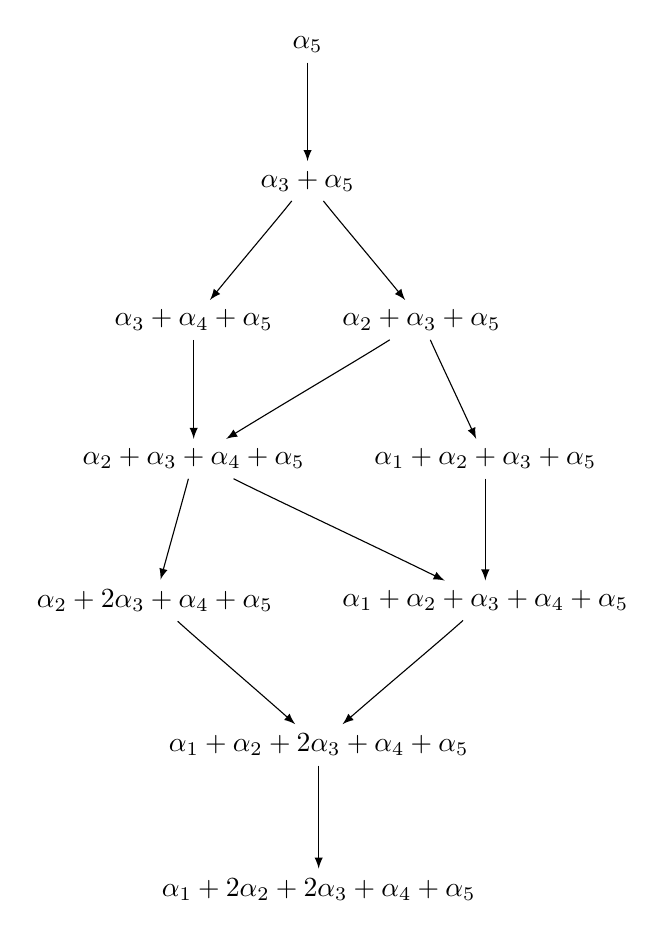
\begin{tikzpicture}[>=latex,line join=bevel,]
%%
\node (alpha2+alpha3+alpha4+alpha5) at (60bp,163bp) [draw,draw=none] {$\alpha_{2} + \alpha_{3} + \alpha_{4} + \alpha_{5}$};
  \node (alpha2+alpha3+alpha5) at (142bp,213bp) [draw,draw=none] {$\alpha_{2} + \alpha_{3} + \alpha_{5}$};
  \node (alpha5) at (101bp,312bp) [draw,draw=none] {$\alpha_{5}$};
  \node (alpha2+2*alpha3+alpha4+alpha5) at (46bp,112bp) [draw,draw=none] {$\alpha_{2} + 2\alpha_{3} + \alpha_{4} + \alpha_{5}$};
  \node (alpha1+2*alpha2+2*alpha3+alpha4+alpha5) at (105bp,8bp) [draw,draw=none] {$\alpha_{1} + 2\alpha_{2} + 2\alpha_{3} + \alpha_{4} + \alpha_{5}$};
  \node (alpha1+alpha2+alpha3+alpha5) at (165bp,163bp) [draw,draw=none] {$\alpha_{1} + \alpha_{2} + \alpha_{3} + \alpha_{5}$};
  \node (alpha1+alpha2+alpha3+alpha4+alpha5) at (165bp,112bp) [draw,draw=none] {$\alpha_{1} + \alpha_{2} + \alpha_{3} + \alpha_{4} + \alpha_{5}$};
  \node (alpha1+alpha2+2*alpha3+alpha4+alpha5) at (105bp,60bp) [draw,draw=none] {$\alpha_{1} + \alpha_{2} + 2\alpha_{3} + \alpha_{4} + \alpha_{5}$};
  \node (alpha3+alpha5) at (101bp,263bp) [draw,draw=none] {$\alpha_{3} + \alpha_{5}$};
  \node (alpha3+alpha4+alpha5) at (60bp,213bp) [draw,draw=none] {$\alpha_{3} + \alpha_{4} + \alpha_{5}$};
  \draw [black,->] (alpha2+alpha3+alpha4+alpha5) ..controls (56.415bp,149.45bp) and (53.345bp,138.71bp)  .. (alpha2+2*alpha3+alpha4+alpha5);
  \draw [black,->] (alpha5) ..controls (101bp,299.84bp) and (101bp,289.19bp)  .. (alpha3+alpha5);
  \draw [black,->] (alpha2+alpha3+alpha5) ..controls (148.19bp,199.08bp) and (153.34bp,188.33bp)  .. (alpha1+alpha2+alpha3+alpha5);
  \draw [black,->] (alpha3+alpha5) ..controls (89.652bp,248.72bp) and (79.772bp,237.15bp)  .. (alpha3+alpha4+alpha5);
  \draw [black,->] (alpha2+alpha3+alpha4+alpha5) ..controls (90.272bp,147.87bp) and (121.55bp,133.28bp)  .. (alpha1+alpha2+alpha3+alpha4+alpha5);
  \draw [black,->] (alpha3+alpha4+alpha5) ..controls (60bp,199.29bp) and (60bp,189.02bp)  .. (alpha2+alpha3+alpha4+alpha5);
  \draw [black,->] (alpha1+alpha2+alpha3+alpha5) ..controls (165bp,149.38bp) and (165bp,138.47bp)  .. (alpha1+alpha2+alpha3+alpha4+alpha5);
  \draw [black,->] (alpha3+alpha5) ..controls (112.35bp,248.72bp) and (122.23bp,237.15bp)  .. (alpha2+alpha3+alpha5);
  \draw [black,->] (alpha2+alpha3+alpha5) ..controls (118.43bp,198.2bp) and (95.43bp,184.74bp)  .. (alpha2+alpha3+alpha4+alpha5);
  \draw [black,->] (alpha1+alpha2+2*alpha3+alpha4+alpha5) ..controls (105bp,45.763bp) and (105bp,35.065bp)  .. (alpha1+2*alpha2+2*alpha3+alpha4+alpha5);
  \draw [black,->] (alpha2+2*alpha3+alpha4+alpha5) ..controls (62.674bp,96.87bp) and (77.694bp,84.141bp)  .. (alpha1+alpha2+2*alpha3+alpha4+alpha5);
  \draw [black,->] (alpha1+alpha2+alpha3+alpha4+alpha5) ..controls (148.58bp,97.315bp) and (132.92bp,84.265bp)  .. (alpha1+alpha2+2*alpha3+alpha4+alpha5);
%
\end{tikzpicture} 
	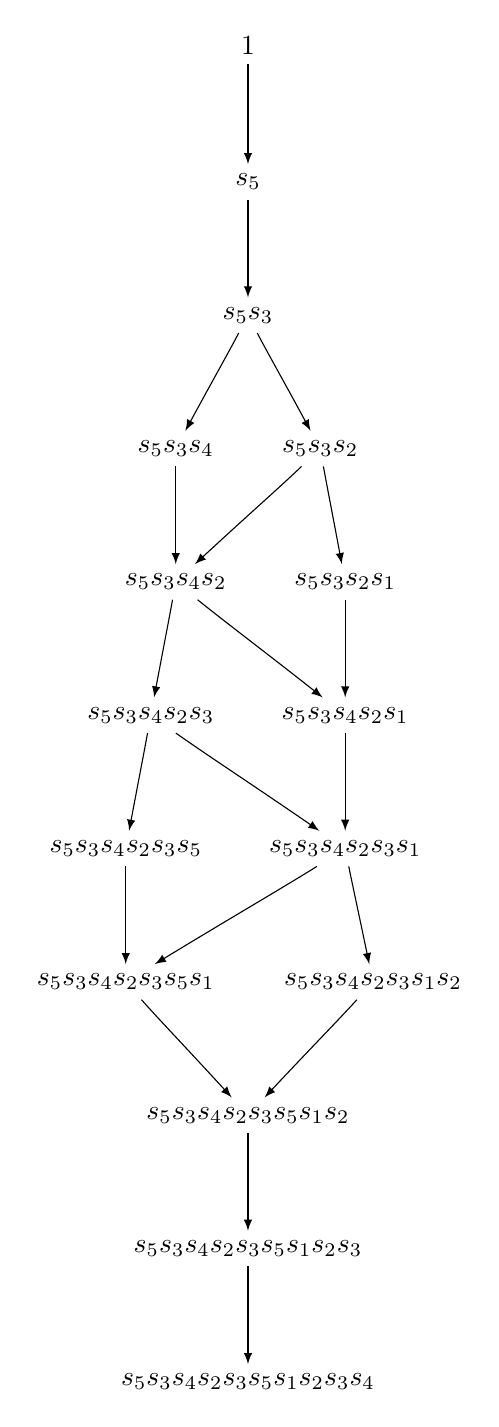
\begin{tikzpicture}[>=latex,line join=bevel,]
%%
\node (s5*s3*s4*s2*s3*s5*s1) at (35bp,150bp) [draw,draw=none] {$s_{5}s_{3}s_{4}s_{2}s_{3}s_{5}s_{1}$};
  \node (s5*s3*s4) at (53bp,342bp) [draw,draw=none] {$s_{5}s_{3}s_{4}$};
  \node (s5*s3*s2) at (105bp,342bp) [draw,draw=none] {$s_{5}s_{3}s_{2}$};
  \node (s5*s3*s2*s1) at (114bp,294bp) [draw,draw=none] {$s_{5}s_{3}s_{2}s_{1}$};
  \node (s5*s3*s4*s2*s3*s1*s2) at (124bp,150bp) [draw,draw=none] {$s_{5}s_{3}s_{4}s_{2}s_{3}s_{1}s_{2}$};
  \node (s5) at (79bp,438bp) [draw,draw=none] {$s_{5}$};
  \node (s5*s3*s4*s2) at (53bp,294bp) [draw,draw=none] {$s_{5}s_{3}s_{4}s_{2}$};
  \node (1) at (79bp,487bp) [draw,draw=none] {$1$};
  \node (s5*s3*s4*s2*s3*s5*s1*s2*s3) at (79bp,54bp) [draw,draw=none] {$s_{5}s_{3}s_{4}s_{2}s_{3}s_{5}s_{1}s_{2}s_{3}$};
  \node (s5*s3*s4*s2*s3*s5) at (35bp,198bp) [draw,draw=none] {$s_{5}s_{3}s_{4}s_{2}s_{3}s_{5}$};
  \node (s5*s3*s4*s2*s3*s5*s1*s2) at (79bp,102bp) [draw,draw=none] {$s_{5}s_{3}s_{4}s_{2}s_{3}s_{5}s_{1}s_{2}$};
  \node (s5*s3*s4*s2*s3*s1) at (114bp,198bp) [draw,draw=none] {$s_{5}s_{3}s_{4}s_{2}s_{3}s_{1}$};
  \node (s5*s3*s4*s2*s1) at (114bp,246bp) [draw,draw=none] {$s_{5}s_{3}s_{4}s_{2}s_{1}$};
  \node (s5*s3) at (79bp,390bp) [draw,draw=none] {$s_{5}s_{3}$};
  \node (s5*s3*s4*s2*s3) at (44bp,246bp) [draw,draw=none] {$s_{5}s_{3}s_{4}s_{2}s_{3}$};
  \node (s5*s3*s4*s2*s3*s5*s1*s2*s3*s4) at (79bp,6bp) [draw,draw=none] {$s_{5}s_{3}s_{4}s_{2}s_{3}s_{5}s_{1}s_{2}s_{3}s_{4}$};
  \draw [black,->] (s5*s3*s4) ..controls (53bp,329.55bp) and (53bp,319.07bp)  .. (s5*s3*s4*s2);
  \draw [black,->] (s5*s3*s4*s2*s3*s1*s2) ..controls (112.12bp,136.86bp) and (100.18bp,124.66bp)  .. (s5*s3*s4*s2*s3*s5*s1*s2);
  \draw [black,->] (s5*s3*s4*s2*s3*s5*s1) ..controls (46.546bp,136.93bp) and (58.051bp,124.9bp)  .. (s5*s3*s4*s2*s3*s5*s1*s2);
  \draw [black,->] (s5*s3*s2) ..controls (107.24bp,329.55bp) and (109.29bp,319.07bp)  .. (s5*s3*s2*s1);
  \draw [black,->] (s5*s3*s2*s1) ..controls (114bp,281.55bp) and (114bp,271.07bp)  .. (s5*s3*s4*s2*s1);
  \draw [black,->] (s5*s3*s4*s2) ..controls (50.76bp,281.55bp) and (48.709bp,271.07bp)  .. (s5*s3*s4*s2*s3);
  \draw [black,->] (s5*s3*s4*s2*s3) ..controls (62.738bp,232.69bp) and (83.077bp,219.32bp)  .. (s5*s3*s4*s2*s3*s1);
  \draw [black,->] (s5*s3*s4*s2*s3*s1) ..controls (116.49bp,185.55bp) and (118.77bp,175.07bp)  .. (s5*s3*s4*s2*s3*s1*s2);
  \draw [black,->] (s5*s3*s4*s2*s3*s5*s1*s2*s3) ..controls (79bp,41.554bp) and (79bp,31.067bp)  .. (s5*s3*s4*s2*s3*s5*s1*s2*s3*s4);
  \draw [black,->] (s5*s3*s4*s2) ..controls (69.466bp,280.58bp) and (86.602bp,267.66bp)  .. (s5*s3*s4*s2*s1);
  \draw [black,->] (s5*s3*s4*s2*s3*s5) ..controls (35bp,185.55bp) and (35bp,175.07bp)  .. (s5*s3*s4*s2*s3*s5*s1);
  \draw [black,->] (s5*s3*s2) ..controls (91.199bp,328.79bp) and (77.201bp,316.41bp)  .. (s5*s3*s4*s2);
  \draw [black,->] (s5*s3*s4*s2*s3*s1) ..controls (92.617bp,184.55bp) and (69.021bp,170.81bp)  .. (s5*s3*s4*s2*s3*s5*s1);
  \draw [black,->] (s5*s3) ..controls (72.374bp,377.28bp) and (66.065bp,366.12bp)  .. (s5*s3*s4);
  \draw [black,->] (s5*s3*s4*s2*s3) ..controls (41.76bp,233.55bp) and (39.709bp,223.07bp)  .. (s5*s3*s4*s2*s3*s5);
  \draw [black,->] (1) ..controls (79bp,473.83bp) and (79bp,463.21bp)  .. (s5);
  \draw [black,->] (s5*s3*s4*s2*s3*s5*s1*s2) ..controls (79bp,89.554bp) and (79bp,79.067bp)  .. (s5*s3*s4*s2*s3*s5*s1*s2*s3);
  \draw [black,->] (s5*s3*s4*s2*s1) ..controls (114bp,233.55bp) and (114bp,223.07bp)  .. (s5*s3*s4*s2*s3*s1);
  \draw [black,->] (s5*s3) ..controls (85.626bp,377.28bp) and (91.935bp,366.12bp)  .. (s5*s3*s2);
  \draw [black,->] (s5) ..controls (79bp,425.55bp) and (79bp,415.07bp)  .. (s5*s3);
%
\end{tikzpicture} 
  \caption{Poset of noncompact roots and the BGG graph for $\mathrm{SO}^*(10)$}
\end{figure} 
